\documentclass[fleqn]{beamer}

\usepackage{amsmath}
\usepackage{animate}
\usepackage{amsfonts}
\usepackage[mathscr]{eucal}
\usepackage{subcaption}
\usepackage{wrapfig}
\usepackage{graphicx}

\usepackage{fancyhdr}
\usepackage{pstricks}
\usepackage{pst-func}
\usepackage{pst-plot}
\usepackage[utf8x]{inputenc}
\usepackage[spanish]{babel}


\setbeamertemplate{navigation symbols}{}
\definecolor{UniBlue}{RGB}{83,121,170}
\setbeamercolor{frametitle}{fg=black,bg=white}
\setbeamercolor{title}{fg=black,bg=yellow!85!orange}
%\setbeamercolor{title}{fg=red,bg=yellow!90!blue}
\usetheme{Madrid}

\beamersetuncovermixins{\opaqueness<1>{25}}{\opaqueness<2->{15}}
\begin{document}

\title{Sistemas Coordenados}
\author{Reynaldo Martell}
\date{\today} 

\begin{frame}
\titlepage
\end{frame}

\begin{frame}\frametitle{\rule{0mm}{10mm}\rule{5mm}{0mm} Sistemas Coordenados. }
\begin{itemize}
\item Desde que a OpenGL se le proporcionan coordenadas 3D hasta que aparecen en la pantalla, las coordenadas espaciales pasan por diferentes sistema de referencia.
\item La transición entre los diferentes sistemas de referencia se lleva a cabo mediante transformaciones que se realizan antes de mostrarse en pantalla.
\item La ventaja de realizar las transformaciones entre cada sistema coordenados se debe a que pueden hacer fácilmente ciertas operaciones en un sistema coordenados.
\item Normalmente existen 5 tipos de sistemas coordenados.
\begin{itemize}
\item Local space (Object space).
\item World space.
\item View space.
\item Clip space.
\item Screen space.
\end{itemize}
\end{itemize}
\end{frame}

\begin{frame}\frametitle{\rule{0mm}{10mm}\rule{5mm}{0mm} Transformaciones entre sistemas de coordenadas. }
\begin{figure}[H]
	\centering
	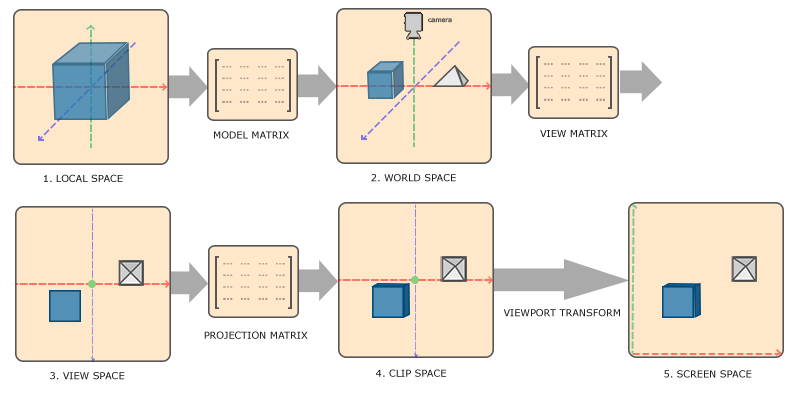
\includegraphics[width=0.95\textwidth]{images/SistemasCoordenados.png}
	\label{mapa}
\end{figure}
\end{frame}

\begin{frame}\frametitle{\rule{0mm}{10mm}\rule{5mm}{0mm} Local Space. }
\begin{itemize}
\item Es el sistema de coordenadas relativo a su origen, es donde el objeto empieza.
\item Imaginar que empezamos a modelar un cubo, el origen del cubo probablemente este en (0, 0, 0)
\item Todos los vértices están referidos al sistema local, origen del modelo.
\item En nuestros ejemplos el rango que se han explicado, los rectángulos están en el rango de –0.5, 0.5 en el origen 0.
\end{itemize}
\end{frame}

\begin{frame}\frametitle{\rule{0mm}{10mm}\rule{5mm}{0mm} World Space. }
\begin{itemize}
\item Imaginar cuando queremos importar nuestros objetos, todos ellos se desplegaran uno encima de otro es decir su origen es (0, 0, 0).
\item Lo deseado es definir una posición para cada objeto que estén en un mundo mas grande.
\item Todas las coordenadas son relativas al mundo.
\item Colocar el objeto en escala, posición y orientación.
\item Las coordenadas locales del objeto son transformados al sistema de coordenadas del mundo mediante una matriz llamada model matrix.
\item Model matrix es una matriz que escala, traslada y rota los objetos en un lugar del mundo.
\end{itemize}
\end{frame}

\begin{frame}\frametitle{\rule{0mm}{10mm}\rule{5mm}{0mm} View Space }
\begin{itemize}
\item El espacio del observador es lo que a menudo se refiera a la cámara de OpenGL.
\item A veces se refiere como espacio de la cámara. 
\item Todas las coordenadas son relativas al mundo.
\item El espacio del observador es el resultado de transformar del sistema de coordenadas del mundo a lo que está enfrente del usuario.
\item Esto se realiza regularmente con trasladar/rotar la escena enfrente de la cámara.
\item La combinación de las transformaciones que se realizan para posicionar los objetos enfrente de la cámara se almacena en una matriz llamada view matrix.
\end{itemize}
\end{frame}

\begin{frame}\frametitle{\rule{0mm}{10mm}\rule{5mm}{0mm} Clip Space }
\begin{itemize}
\item OpenGL espera que los vértices se encuentran en un rango de valores.
\item Los valores que no se encuentren en este rango son recortados y descartados del renderizado.
\item Esto es conocido como clip space.
\item Regularmente lo que se hace es manejar nuestro propio espacio de recorte por ejemplo –100 a 100 y después aplicarle una transformación para que sean recortadas las coordenadas en el espacio de –1 a 1.
\item La matriz que llamaremos matriz del proyección es la que especifica este rango para posteriormente hacer la normalización.
\end{itemize}
\end{frame}

\begin{frame}\frametitle{\rule{0mm}{10mm}\rule{5mm}{0mm} Clip Space }
\begin{itemize}
\item Por ejemplo si la matriz de proyección especifica un rango entre -1000 a 1000 el punto (1250, 500, 750) no será visible debido a que x no esta en el rango de 1000 a 1000.
\item Si una primitiva por ejemplo un triangulo esta fuera del volumen de recorte OpenGL reconstruye el triangulo para que muestra el pedazo que cae dentro del volumen de recorte.
\item Este volumen de recorte es comúnmente llamado Frustum.
\item Todas las coordenadas que se encuentran dentro de la caja del Frustum son mostrados en pantalla.
\end{itemize}
\end{frame}

\begin{frame}\frametitle{\rule{0mm}{10mm}\rule{5mm}{0mm} Clip Space }
\begin{itemize}
\item Una  vez que todos los vértices son transformados al espacio de recorte se realiza una operación final llamada perspective division.
\item Esta operación consiste en dividir las coordenadas x, y y z del vector por la componente w de su coordenada homogénea.
\end{itemize}
\end{frame}

\begin{frame}\frametitle{\rule{0mm}{10mm}\rule{5mm}{0mm} Screen Space }
\begin{itemize}
\item Después las coordenadas son mapeadas a coordenadas de la pantalla usando glViewport().
\end{itemize}
\end{frame}

\begin{frame}\frametitle{\rule{0mm}{10mm}\rule{5mm}{0mm} Proyecciones }
\begin{itemize}
\item Las proyecciones se encargan de realizar el proceso de recorte y de convertir la información de los vértices de la escena a coordenadas en dos dimensiones.
\item Existen varias propiedades que se le asocian a una proyección y de estás depende como se visualizara nuestra escena.
\end{itemize}
\end{frame}

\begin{frame}\frametitle{\rule{0mm}{10mm}\rule{5mm}{0mm} Tipos de proyecciones }
\begin{itemize}
\item Proyección ortogonal.
\item Proyección en perspectiva.
\end{itemize}
\end{frame}

\begin{frame}\frametitle{\rule{0mm}{10mm}\rule{5mm}{0mm} Elementos de una proyección }
Si importar cual sea el tipo de proyección, ambas tienen los siguientes elementos:
\begin{itemize}
\item Punto focal o punto de proyección: Lugar geométrico donde se encuentra el origen de apertura de proyección (Origen del observador).
\item Líneas de proyección. Son líneas rectas que van desde el origen de apertura de la proyección a los vértices de la geometría.
\item Plano de proyección: Plano que se encuentra entre el punto en coordenadas espaciales y el punto focal.
\item Volumen de proyección. Es el espacio en el cual se visualiza nuestra escena.
\end{itemize}
\end{frame}

\begin{frame}\frametitle{\rule{0mm}{10mm}\rule{5mm}{0mm} Elementos de una proyección }
\begin{figure}[htb]
	\centering
	\begin{tabular}{@{}cccc@{}}
	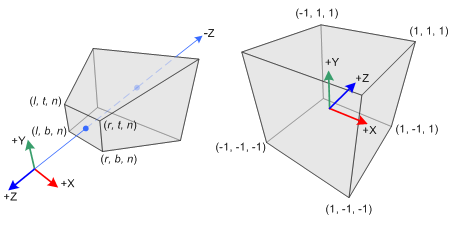
\includegraphics[width=.64\textwidth]{images/ElementosProyeccion1.png} &
    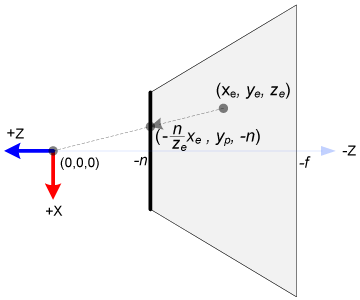
\includegraphics[width=.34\textwidth]{images/ElementosProyeccion2.png} &
	\end{tabular}
	\label{mapa}
\end{figure}
\end{frame}

\begin{frame}\frametitle{\rule{0mm}{10mm}\rule{5mm}{0mm} Proyección ortogonal }
\begin{itemize}
\item La matriz de una proyección ortogonal define una especie de caja como frustum, la cual define el espacio de recorte.
\item Los vértices que quedan fuera de la caja son recortados.
\item Para especificar la matriz de proyección ortográfica es necesario definir ancho, alto y largo del frustum.
\end{itemize}
\end{frame}

\begin{frame}\frametitle{\rule{0mm}{10mm}\rule{5mm}{0mm} Proyección ortogonal }
\begin{figure}[H]
	\centering
	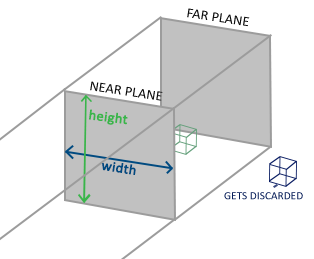
\includegraphics[width=0.65\textwidth]{images/ortogonal.png}
\end{figure}
\end{frame}

\begin{frame}\frametitle{\rule{0mm}{10mm}\rule{5mm}{0mm} Proyección ortogonal }
\begin{figure}[H]
	\centering
	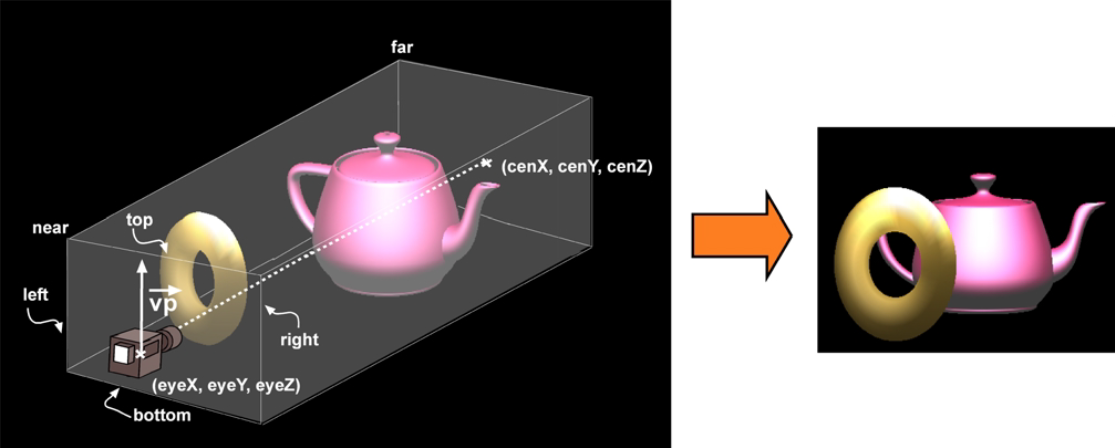
\includegraphics[width=0.95\textwidth]{images/ortogonal2.png}
\end{figure}
\end{frame}

\begin{frame}\frametitle{\rule{0mm}{10mm}\rule{5mm}{0mm} Matrix de Proyección ortogonal }
\centering
$
M_{ortogonal} = 
\begin{bmatrix}
\frac{2}{r-l} & 0 & 0 & -\frac{r+l}{r-l} \\
0 & \frac{2}{t-b} & 0 & -\frac{t+b}{t-b} \\
0 & 0 & \frac{-2}{f-n} & -\frac{f+n}{f-n} \\
0 & 0 & 0 & 1
\end{bmatrix}
$
\end{frame}

\begin{frame}\frametitle{\rule{0mm}{10mm}\rule{5mm}{0mm} Proyección ortogonal OpenGL }
\begin{itemize}
\item Para crear la matriz de proyección ortográfica.
\\
\textbf{glm::ortho(-1.0f, 1.0f, -1.0f, 1.0f, 0.1f, 100.0f);}

\item Los primeros dos parámetros especifican las coordenadas izquierda y derecha del frustrm.
\item Los parámetros 3 y 4 especifican la parte inferior y superior.
\item Los parámetros 5 y 6 especifican la distancia entre el plano cercano y plano lejano.
\end{itemize}
\end{frame}

\begin{frame}\frametitle{\rule{0mm}{10mm}\rule{5mm}{0mm} Proyección en perspectiva }
\begin{itemize}
\item En gráficos para computadora el efecto de perspectiva se da cuando los objetos que están mas lejos de la escena aparecen mas pequeños. 
\item Esta técnica es usada para darle profundidad a los objetos.
\item La matriz de proyección no solo mapea las coordenadas a un rango de valores al espacio de recorte.
\item También manipula el valor w de cada vértice, de tal forma que los vértices que se encuentran mas alejados en profundidad z aparecen mas lejanos. 
\end{itemize}
\end{frame}

\begin{frame}\frametitle{\rule{0mm}{10mm}\rule{5mm}{0mm} Proyección en perspectiva }
\begin{figure}[htb]
	\centering
	\begin{tabular}{@{}cccc@{}}
	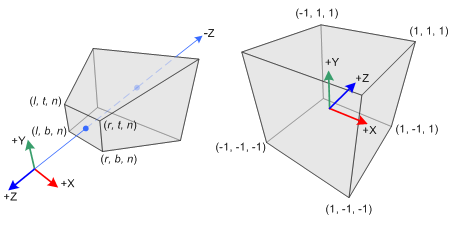
\includegraphics[width=.64\textwidth]{images/ElementosProyeccion1.png} &
    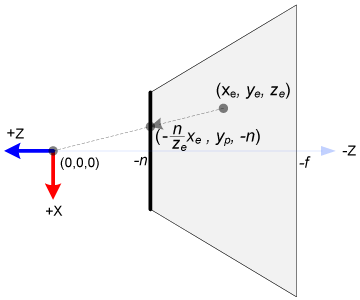
\includegraphics[width=.34\textwidth]{images/ElementosProyeccion2.png} &
	\end{tabular}
	\label{mapa}
\end{figure}
\end{frame}

\begin{frame}\frametitle{\rule{0mm}{10mm}\rule{5mm}{0mm} Proyección en perspectiva }
\begin{figure}[H]
	\centering
	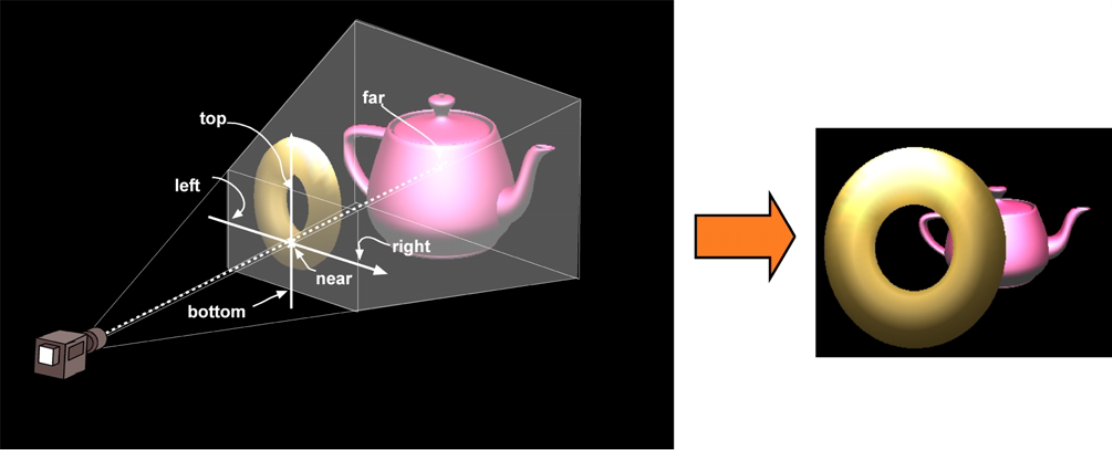
\includegraphics[width=0.95\textwidth]{images/perspectiva.png}
\end{figure}
\end{frame}

\begin{frame}\frametitle{\rule{0mm}{10mm}\rule{5mm}{0mm} Matrix de Proyección en perspectiva }
\centering
$
M_{perspective} = 
\begin{bmatrix}
\frac{2n}{r-l} & 0 & \frac{r+l}{r-l} & 0 \\
0 & \frac{2n}{t-b} & \frac{t+b}{t-b} & 0 \\
0 & 0 & \frac{-(f+n)}{f-n} & \frac{-2fn}{f-n} \\
0 & 0 & -1 & 0
\end{bmatrix}
$
\end{frame}

\begin{frame}\frametitle{\rule{0mm}{10mm}\rule{5mm}{0mm} Proyección en perspectiva OpenGL }
\begin{itemize}
\item La matriz en perspectiva también se puede crear con glm de la siguiente manera.
\\
\textbf{glm::perspective(45.0f, (float)width/(float)height, 0.1f, 100.0f);}

\item \textbf{glm::perspective} crea una pirámide que define el espacio visible.
\item Todo lo que quede fuera de este volumen es recortado.
\item El primer parámetro define el field of view (FOV).
\item El segundo parámetro es el aspect ratio que se calcula dividiendo el ancho y alto de la pantalla.
\item El tercer y cuarto parámetro es la distancia que existe en el plano cercano y plano lejano. en perspectiva.
\end{itemize}
\end{frame}

\end{document}